\section{Examples of Adding Graphics}
\label{Sec:addingGraphics}
All of the below code with subfigures A-Z was generated with:
\begin{verbatim}
\begin{multiFigure}
\addFigure{0.3}{./theworld.png}
\addFigure{0.2}{./theworld.png}
\addFigure{0.4}{./theworld.png}
\addFigure[Z]{0.6}{./theworld.png}
\captionof{figure}[This is a test caption.]{This is a test caption. 
This text has the bit for the whole figure.  Meanwhile, subfigure A is weird 
looking map. Subfigure B is a smaller map. And Subfigure C 
is a bigger but still weird looking map. 
Moreover, I can override the map, which is why Z is 
another weird map that came after map C.}
\end{multiFigure}
\end{verbatim}
Note that \LaTeX{} can be fickle when it comes to placing figures relative to text near the figure. Specifically, the ``Figure" environment is a `float' type, which is placed somewhere ``nearby" where it appears in the text, which can be pretty frustrating. For this reason we have circumvented the `float' part of the figure in order to allow more control over the figure placement. 

If one uses the \verb|\begin{figure}\end{figure}| construction, the figure may appear in a odd place, whereas you can use the \verb|\begin{multiFigure}\end{multiFigure}| even with only 1 figure, to force placement to work. When using multiFigure captions need to be placed using the command \verb|\captionof{<NAME>}[<LIST-ENTRY>]{<CAPTION>}| where NAME is the type of caption, LIST-ENTRY is what appears in the `List of' at the beginning of the thesis, and CAPTION is the actual caption. For single image figures, it will be better to use the \verb|\begin{figure}\end{figure}| construction was the Graduate Editorial Office does not need a letter-label, for a figure with only one image. 

\begin{flushleft}
    \begin{multiFigure}
        \begin{center}
            \addFigure{0.3}{graphics/theworld.png}
            \addFigure{0.2}{graphics/theworld.png}
            \addFigure{0.4}{graphics/theworld.png}
            \addFigure[Z]{0.6}{graphics/theworld.png}
        \end{center}
\captionof{figure}[This is my shortened caption for my Table of Contents]{This is a test caption. This text has the bit for the whole figure. Meanwhile, subfigure A is weird looking map. Subfigure B is a smaller map. And Subfigure C is a bigger but still weird looking map. Moreover, I can override the map, which is why Z is another weird map that came after map C.}
\end{multiFigure}
\end{flushleft}


\begin{figure}[h!]
    \begin{center}
        \includegraphics[width=0.9\textwidth]{graphics/theworld.png}
    \end{center}
     \caption[This is my shortened caption for my Table of Contents] {This is a super-long caption to make sure that the caption in the list-of section is correctly single space with the blank white line between captions. That being said, you should probably always use the list-entry optional argument in the captionof command to write a shorter caption instead of this nonsense.}
\end{figure}

\section{A Note on Graphics}
The command \verb|\addFigure| in the multiFigure environment, and/or the command \verb|\includegraphics| will take almost every type of graphic file currently in use as of the writing of this template. The only notable exception is the bitmap, ie .bmp file. Most software won't save to bitmap without specifically requesting it at this point, but if you have generated a .bmp file you can load it in most any graphic editor (eg MSpaint or photoshop) and save it as a different file type, such as .PNG which is significantly smaller file size as well. Note that the commands typically require the file extension to be included, and it is case sensitive. Thus in the above \verb|\addFigure{0.2}{./theworld.png}| works but \verb|\addFigure{0.2}{./theworld.PNG}| would error and \verb|\addFigure{0.2}{./theworld}| may or may not work depending on which specific TeX editor you are using.

\section{Placement Specifiers}

Floats are used to allow LaTeX to handle figures while maintaining the best possible presentation. However, there may be times when you disagree, and a typical example is with its positioning of figures. The placement specifier parameter exists as a compromise, and its purpose is to give the author a greater degree of control over where certain floats are placed. 


\begin{table}[H]
\caption{Specifier Table}
\begin{tabular}{l p{14cm} }
\hline
Specifier & Permission \\ \hline
h & Place the float here, i.e., approximately at the same point it occurs in the source text (however, not exactly at the spot) \\
\\
t & Position at the top of the page.  \\
\\
b & Position at the bottom of the page.  \\
\\
p & Put on a special page for floats only.  \\
\\
! & Override internal parameters LaTeX uses for determining "good" float positions. \\
\\
H & Places the float at precisely the location in the LaTeX code. \\
\hline
\end{tabular}
\end{table}

An example of a specifier parameter is shown below to force a figure into place where it is mentioned in text: 

\begin{verbatim}
\begin{figure}[h!]
    \begin{center}
        \includegraphics[width=0.9\textwidth]{./theworld.png}
    \end{center}
     \caption[My short caption.]{My full caption in curly brackets.}
\end{figure}
\end{verbatim}